%%%%%%%%%%%%%%%%%%%%
%\section{Heavy-flavour multiquark states}

\section{Experimental evidences of heavy-flavour multiquark candidates}
\label{subsection:experimental_introduction}


\subsection{Neutral $X$ and $Y$ multiquark candidates}

\subsubsection{First tetraquark candidate \theX}

The first multiquark candidate is \theX, 
which was observed by Belle Collaboration as a narrow peak in the $\pip\pim\jpsi$ invariant mass distribution 
$B\to K\pip\pim\jpsi$ decays for in 2003\supercite{PhysRevLett.91.262001}.
The invariant mass distribution of $B\to K\pip\pim\jpsi$ is shown in Figure.~\ref{fig:X3872_BELLE},
this resonance is pretty narrow and close to the threshold of the $\D\Dstarb$,
it was popular to be assumed as molecular state,
though the dynamic mechanism is under heated debate today. 
As this state has been discovered more than 16 years, 
and comfirmed in different experiments,
the related studies are pretty fruitful in experimental and theoritical sectors,
some comments about this paritlce will be given below.


\begin{figure}[!hbtp]
\centering
\includegraphics[width=0.9\textwidth]{Figures/01_Introduction/Exotic/X3872_BELLE}%
\caption{Signal-band projections of (a) $M_{bc}$, (b) $\Delta E_{c.m}$ , and (c) $M(\pip\pim\jpsi)$ distributions in
   signal region with the results of the unbinned fit\supercite{PhysRevLett.91.262001}.}
\label{fig:X3872_BELLE}
\end{figure}

The spin and parity of this state were measured by LHCb Collaboration in 2013 with 3\invfb run-I data\supercite{LHCb-PAPER-2013-001}.
5D angular amplitude model was constructed to discribe data,
and likelihood ratio test is performed to discriminate between the $1^{++}$ and $2^{-+}$ assignment.
Based on this technique,
the quantum numbers of \theX are detemined to be $J^{PC}=1^{++}$,
as shown in Figure.~\ref{fig:X3872_spin}.
By a toy simulation method,
the statistical significance of this asssignment can rearch to $16\sigma$.

\begin{figure}[!hbtp]
\centering
\includegraphics[width=0.6\textwidth]{Figures/01_Introduction/Exotic/X3872_Spin}%
   \caption{ The log-likelihood ratio distribution between $1^++$ and $2^{-+}$ is shown above,
   a Gaussian fit to the $2^{-+}$ distribution is performed\supercite{LHCb-PAPER-2013-001}.}
\label{fig:X3872_spin}
\end{figure}

As the spin and parity of \theX equel to $1^{+}$,
this hadron is also expected as $2^{3}P_{1}$ $c\bar{c}$ state.
However, 
there are still several reasons to classify it as exotic state\supercite{Olsen:2017bmm},
and the apparent evidence is isospin violation in its decay channel $\theX\to\rho\jpsi$.
Since the standard charmonium states contain no constituent \uquark or \dquark,
their isospin number should be 0,
as the $\rho$ is isovector particle, 
the decay mode $\theX\to\rho\jpsi$ should be strongly suppressed due to isospin violation, 
but branching fraction of this decay is nearly equal to the $\theX\to\omega\jpsi$ mode.
In consideration of a kinematic suppression to $\theX\to\omega\jpsi$ by a factor of around 4,
the $I=0$ assignment is favored.

Many explorations to the nature of \theX were performed by different theoretical models\supercite{LIU2019237},
and a good diagnosis to these predictions is to study the relative strength to the $\gamma\psi$ and $\gamma\jpsi$ decay modes.
In the $1^{++}$ charmonium model, 
the $\chicone^{'}$ and $\psi^{'}$ have the same redial wave function,
and $\chicone^{'}\to\gamma\psi^{'}$ transition is more advantageous than that for $\gamma\jpsi$.
In contrast,
in the molecular hypothesis,
the decay to $\gamma\psi^{'}$ is much suppressed\supercite{SWANSON2004189,SWANSON2004197,Dong_2010}.
The evidence for the decay mode $\chicone^{'}\to\gamma\psi^{'}$ was found in 2014, 
and the measured value agrees with expectations of charmonium for pure interpretation of the $\theX$ state
and mixture of charmonium interpretations,
it does not support a pure $\D\Dstarb$ molecular interpretation\supercite{LHCb-PAPER-2014-008}.

Another experimental test to distiguish hypothesis is to measure the prompt production of \theX in high-energy hadron collisions.
If the \theX is a $\D\Dstarb$ state,
its production in the hadron collisions would be more like those of known nuclei stuff, 
rather than those of the $\psi^{'}$\supercite{PhysRevLett.103.162001}.


\subsubsection{$X(3915)$}

After the \theX was observed,
Belle Collaboration studied $B\to K\omega\jpsi$ decay,
and a prominent enhancement appeared in the $\omega\jpsi$ invariant mass distribution near the threshold,
as shown in Figure.~\ref{fig:X3915}(a).
Then,
\babar Collaboration confirmed this result with larger statistic sample,
and the measured mass and width : $M=3915\pm4\mev$ and $\Gamma=31\pm11\mev$,
which are lower values comparing to Belle's measurement\supercite{PhysRevD.82.011101}.
Then,
this state was also observed in the two-photon process $\gamma\gamma\to\omega\jpsi$, 
and the PDG table list the results from both channels\supercite{PDG2020}.

\begin{figure}[!hbtp]
\centering
   \includegraphics[width=0.32\textwidth]{Figures/01_Introduction/Exotic/X3915_BELLE}%
   %\put(-60,168) {\textrm{\small \bf(a)}}
   \includegraphics[width=0.4\textwidth]{Figures/01_Introduction/Exotic/X3915_BABAR}%
   %\put(10,168) {\textrm{\small \bf(b)}}
   \caption{ The decay $X(3915)\to\omega\jpsi$ states in $B\to K\omega\jpsi$ decay from \belle\supercite{PhysRevLett.103.162001} (left),
   and \babar\supercite{PhysRevD.82.011101} (right).}
\label{fig:X3915}
\end{figure}

However,
the spin-parity of this state has not been confirmed yet.
With the $\g\g\to\omega\jpsi$ events,
a spin-parity analysis was performed by \babar,
and their study demonstrated that $J^{PC}=0^{++}$ quantum number assignment is favoured.
And from this study,
they thought the $X(3915)$ is a candidate for the $2^{3}\rm{P}_{0}$ charmonium state\supercite{PhysRevLett.104.092001}.
This measured mass of $X(3915)$ is too high for the $2^{3}\rm{P}_{0}$ charmonium state,
which is strongly contradicted with theoretical expectations\supercite{PhysRevD.69.094019,PhysRevD.79.094004}.

Besides,
some people think the $J^{PC}=2^{++}$ hypothesis cannot be ruled out by reanalying from the \babar angular distributions\supercite{PhysRevLett.115.022001}.
However,
$X(3915)=\chi_{c2}^{'}$ is not in accordance with the consquence of $X(3915)$ productiojn in $\Bp\to\Kp\omega\jpsi$ decay.
Since that $\BF(\Bp\to\Kp\chictwo(1\rm{P})) = (1.1\pm0.4)\times10^{-5}$ is much smaller than the branching fraction of:
\begin{equation}
\BF(\Bp\to\Kp X(3915))\times\BF(X\to\omega\jpsi)=3.0^{+0.9}_{-0.7}\times10^{-5}
\label{eq:X_3915_BF}
\end{equation}
In the decay of B-meson to charmonium states, 
the decay widths are expected to be proportional to the square of the $\cquark\cquarkbar$ wave function at the origin,
and decrease with increasing radial quantum number\supercite{PhysRevD.46.R3703}.
The branching fraction measurement is contrary to this model obviously.

The mass of $X(3915)$ is $18.2 \mev$ below the $2m_{\Ds}$ threshold,
and this might mean that it consists of $\cquark\cquarkbar\squark\squarkbar$ component,
or even in a $\Dsp\Dsm$ melecule-like situation.
In the molecular picture,
the $\D\Dbar$ decay would vilolate the OZI-rule\supercite{PhysRevD.59.114027}.
In the $\cquark\cquarkbar\squark\squarkbar$ configuration,
the decay mode least affected by OZI-suppression is $X(3915)\to\eta\etac$ which could be expected to be a dominant decay mode.
However,
\belle saw no significant signal from previous study\supercite{Vinokurova:2015txd}.
The absence of an $\eta\etac$ model would be fatal teh $\cquark\cquarkbar\squark\squarkbar$ quark assignment 
if its partial width was shown to be definately much smaller than that for $\omega\jpsi$ decays.


The $X(3915)$ is one of the most intriguing of the $XYZ$ exotic meson candidates,
however, 
its underlying nature is not fully understood,
and larger data sample of this state is required in the future experiments.
The $J^{P}$ of this state is expected to be detemined from \belletwo,
which have a good ability to reconstruct $\omega$ meson.
Besides,
\lhcb experiment also has potential capacity to probe the $X(3915)$ quantum number,
considering the $\omega$ has been detected in \Bp decay\supercite{LHCb-PAPER-2012-022}.


\subsubsection{$X(4140)$ and other $\jpsi\phi$ states}

Among all known decays of $b-$hadrons,
$\Bp\to\jpsi\phi K^+$ is unique, 
since conventional hadron contributions from kaon excitations (hereafter denoted as $K^{*+}\to\phi K^+$) are broad, 
and visible mass structures on the Dalitz plot are dominated by a number of relatively narrow $X\to\jpsi\phi$ states, 
which are candidates for tetraquarks with hidden-charm and hidden-strangeness. 
Contributions from these exotic hadron components approach half of the entire rate in this decay channel.
The first evidence for the $\jpsi\phi$ state was observed by CDF~\supercite{Aaltonen:2011at},
as shown in the left of Figure.~\ref{newfig3}.
A very narrow ($\Gamma=15.3_{-\phantom{1}6.1}^{+10.4}\pm2.5$\mev), 
near-threshold ($M=4143.4\pm3.0\pm0.6$\mev)
$X(4140)$ state was claimed.
\footnote{The recent PDG\supercite{PDG2020} naming convention calls this state $\chi_{c1}(4140)$. 
However, the generic $X$ label for $\jpsi\phi$ states is used here, 
which is independent of their $J^P$ assignments.}
Such narrow structure was not confirmed by the \belle~\supercite{ChengPing:2009vu}, 
\babar~\supercite{Lees:2014lra}, 
and early low-statistics \lhcb~\supercite{LHCb-PAPER-2011-033} data. 
However, 
the near-threshold state was observed by the \cms collaboration~\supercite{Chatrchyan:2013dma}. 
There was also an evidence for it from the \dzero experiment~\supercite{Abazov:2015sxa},
as shown in the right of Figure.~\ref{fig:D0_4140}.

\begin{figure}[htb]
  \begin{center}
  \vspace{-0.3cm}
   \includegraphics[width=0.41\textwidth]{Figures/01_Introduction/Exotic/neutral_particle/CDF_4140}
   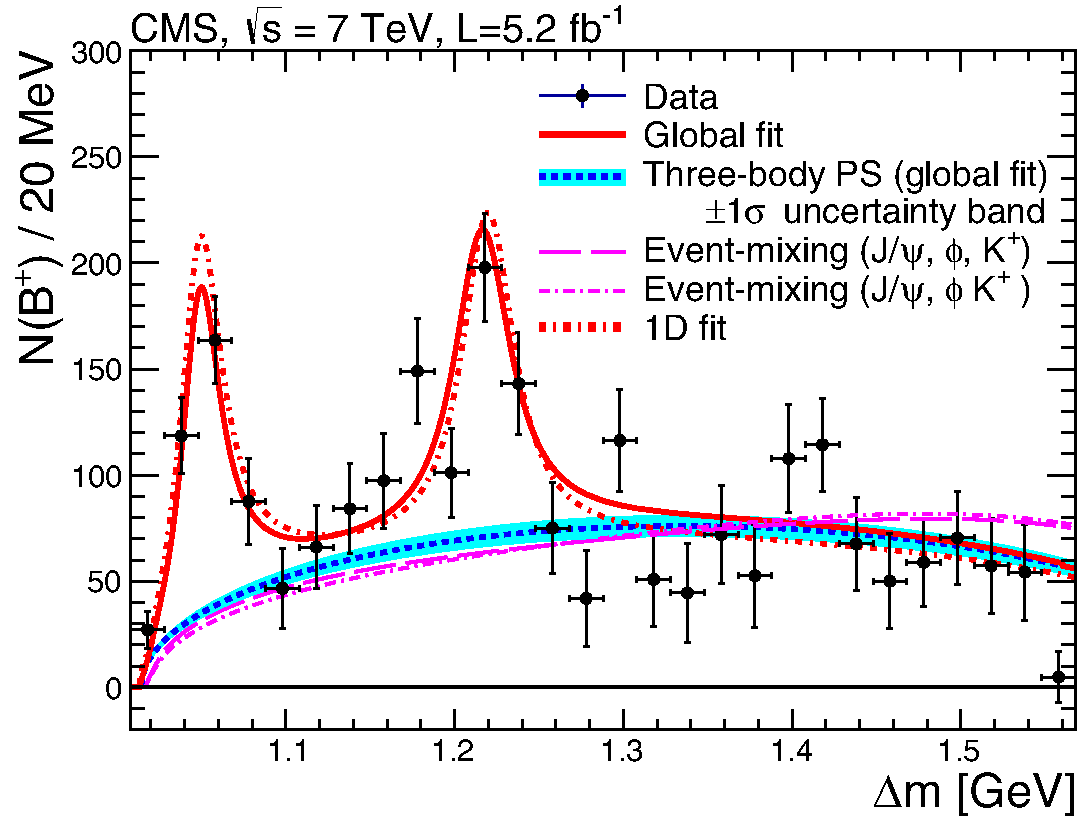
\includegraphics[width=0.48\textwidth]{Figures/01_Introduction/Physics/from_Zcs/newFig3.pdf}
     \vskip -0.4cm
    \caption{\small
     The $\Delta M = M(\jpsi\phi)-M(\jpsi)$ distribution of $\Bp\to\jpsi\phi\Kp$ decays candidates from \cdf experiment in left\supercite{Aaltonen:2011at}; 
     The number of  $\Bp\to\jpsi\phi K^+$  candidates as a function 
     of $\Delta m = m(\mu^+\mu^-\Kp\Km)-m(\mu^+\mu^-)$ at \cms in right\supercite{Abazov:2015sxa}.
    }
    \label{newfig3}
  \end{center}
\end{figure}

\begin{figure}[htb]
  \begin{center}
  \vspace{-0.3cm}
   \includegraphics[width=0.91\textwidth]{Figures/01_Introduction/Exotic/neutral_particle/D0_4140}
     \vskip -0.4cm
    \caption{\small
     The $\Delta M = M(\jpsi\phi)-M(\jpsi)$ distribution of $\Bp\to\jpsi\phi\Kp$ decays candidates from \cdf experiment in left\supercite{Aaltonen:2011at}; 
     The number of  $\Bp\to\jpsi\phi K^+$  candidates as a function 
     of $\Delta m = m(\mu^+\mu^-\Kp\Km)-m(\mu^+\mu^-)$ at \cms in right\supercite{Abazov:2015sxa}.
    }
    \label{fig:D0_4140}
  \end{center}
\end{figure}

An evidence for a second structure, $X(4274)$, in the \cdf\supercite{Aaltonen:2011at} and \cms\supercite{Chatrchyan:2013dma} was observed.
%The \cdf collaboration presented $3.1 \sigma$ evidence for a second relatively narrow $\jpsi\phi$ mass peak around $4274\pm8 \mev$\supercite{}.
The $\jpsi\phi$ mass distribution among $2480\pm160$ $\Bp\to\jpsi\phi K^+$ events detected by \cms is shown in right of Figure.~\ref{newfig3}, 
which was obtained after the subtraction of a very large combinatorial background.
There is also hint of the second structure near $4274 \mev$ in the $\jpsi\phi$ mass distribution at \dzero,
as shown in the left of Figure.~\ref{fig:D0_4140},
with a small significance around $1.7 \sigma$. 
Besides,
\belle reported a $3.2 \sigma$ evidence of a narrow $\jpsi\phi$ peak around $4351 \mev$,
and the corresponding $J^P$ assignment is $0^{++}$ or $2^{++}$.
However, there is no obvious $X(4140)$ evidence in the same sample\supercite{PhysRevLett.104.112004}.


\lhcb~\supercite{LHCb-PAPER-2016-018,LHCb-PAPER-2016-019} performed the first amplitude analysis of $\Bp\to\jpsi \phi K^+$ decays,
by investigating the $\jpsi \phi$ structures in Run 1 data.
The number of $\Bp\to\jpsi \phi K^+$ signal events was $4289\pm141$ with a background fraction of $23\%$.
The data can be described by including seven $K^{*+}\to\phi K^+$ resonances,
which are determined by the fit and consistent with either known or predicted states,
besides, 
four $X\to\jpsi\phi$ structures and non-resonant $\phi K^+$ and $\jpsi \phi$ also contribute.
The mass projections of $\phi K^+$ and $\jpsi \phi$ combinations are shown in Figure.~\ref{fig:defmasses}.
%Table~\ref{tab:run1} shows the results, including the determined masses, widths, fit fractions and spin-parity assignments.
The four $X$ structures and a non-resonant $\jpsi\phi$ contribution all had significance above 5$\sigma$.
The existence of $\Xtwo$ was established.

\begin{figure}[hbtp]
  \begin{center}
    \includegraphics[width=0.5\textwidth]{Figures/01_Introduction/Physics/from_Zcs/newbase_PhiKh.pdf}%
    \includegraphics[width=0.5\textwidth]{Figures/01_Introduction/Physics/from_Zcs/newbase_JpsiPhih.pdf}
  \end{center}
\caption{
    Distributions of $\phi K^+$ (left) and $\jpsi\phi$ (right)
    invariant masses for the $\Bp\to\jpsi \phi K^+$ candidates (black data points)
    compared with the results of the default amplitude fit
    to the Run 1 data \supercite{LHCb-PAPER-2016-018}.}
  \label{fig:defmasses}
\end{figure}

The $J^{P}$ quantum numbers of $\Xone$ are determined to be $1^{++}$.
Besides,
the $\Xtwo$ state were identified as $1^{++}$ at  $>5\sigma$ significance,
while the $\Xthree$ and $\Xfour$ states as $0^{++}$ at $>4\sigma$. 
Actually,
the $1^{++}$ quantum number for $\Xone$ and $\Xtwo$ rule out the $0^{++}$ or $2^{++}$ $\Dss\Dssm$molecular models
%\supercite{PhysRevD.80.017502,PhysRevD.80.054019,Zhang_2010,PhysRevD.80.114013,ALBUQUERQUE2009186,Wang:2009ry,Ding:2009vd}.
\supercite{PhysRevD.80.017502,PhysRevD.80.054019,PhysRevD.80.114013,ALBUQUERQUE2009186,Wang:2009ry,Ding:2009vd}.
Besides,
some people suggested $\Xone$ structure is kinematically induced cusp\supercite{PhysRevD.91.034009,KARLINER2016365}.
No proposed molecular bound-state or cusp model can account for these $\Xtwo J^{PC}$ values. 
A hybrid charmonium state in this mass region would have $J^{PC}=1^{-+}$\supercite{MAHAJAN2009228}.
An exception is a tetraquark model implemented by Stancu\supercite{Stancu_2010},
states that not only correctly assigned $1^{++}$ to the $\Xone$, 
but also predicted a second $1^{++}$ state at a mass that is not much higher than that of the $\Xtwo$.
The $\Xthree$ and the $\Xfour$ have been suggested as candidates for the $\chiczero(4P)$ and $\chiczero(5P)$ states, 
since they lie in the predicted mass and width ranges for these states\supercite{PhysRevD.94.074007,PhysRevD.94.114018}.
However,
none of the \jpsi structures observed in B decays are consistent with the state seen in two-photon collisions by the Belle collaboration.\supercite{PhysRevLett.104.112004}

Notably, the $\Xone$ width was substantially larger than previously determined,
while the mass is consistent with the $\Xone$ values from \cdf and \cms. 
In the spectroscopy study,
a one-dimensional fit to a mass distribution for a resonance peak might lead to biased mass and width.
Besides, 
a one-dimensional fit might underestimate systematic error,
due to the given assumption about the background shape and its incoherence\supercite{RevModPhys.90.015003}.


\begin{table*}[bht]
%\scriptsize  
\caption{Results related to the $X(4140)\to\jpsi\phi$ mass peak,
first observed in $B^+\to\jpsi\phi K^+$ decays.
The first (second) significance quoted for Ref.~[\cite{Abazov:2015sxa}]
is for the non-prompt (prompt) production components (the mass and width were determined from the non-prompt sample).
The last column gives a fraction of $B^+\to\jpsi\phi K^+$ rate
attributed to the $X(4140)$ structure, however, the CDF and
D0 results were normalized to a $B^+\to\jpsi\phi K^+$ rate
that excluded the high $\jpsi\phi$ mass range.
}
\label{tab:x4140}
\hbox{
\hbox{
\renewcommand{\arraystretch}{1.2}
\def\1#1{\multicolumn{1}{c}{#1}}
%\def\2{\ifthenelse{\boolean{prl}}{\quad}{}}
\def\2{}
%\def\3{\ifthenelse{\boolean{prl}}{}{\!\!\!}}
%\def\pms{\ifthenelse{\boolean{prl}}{\pm}{\!\pm\!}}
\begin{tabular}{cllcl}
\hline
%Year & Experiment  & \1{$B\to\jpsi\phi K$} & \multicolumn{4}{c}{$X(4140)$ peak} \\
%     & luminosity  & \1{yield}             & \1{Mass [MeV]} & \1{Width [MeV]} & \1{Significance} & \1{Fraction \%} \\
     {$B\to\jpsi\phi K$} & \multicolumn{4}{c}{$X(4140)$ peak} \\
     {yield}   & {Mass [\mev]} & {Width [\mev]} & {Significance} & {Fraction \%} \\

\hline\hline
2008 &  \multicolumn{3}{l}{\cdf 2.7 fb$^{-1}$  \cite{Aaltonen:2009tz} }\\ \hdashline
$58\pm10$ \2 &
$4143.0\pm2.9\pm1.2$ {\quad} &
$11.7\,^{+8.3}_{-5.0}\pm3.7$ &
$3.8\sigma$ & \\ \hline
%\hline
{\it 2009} & \multicolumn{3}{l}{ {\it \belle} \cite{Brodzicka:2010zz} } \\ \hdashline
$\mathit{325\pm21}$  &
$\mathit{4143.0}$ {\it fixed} &
$\mathit{11.7}$ {\it fixed} &
$\mathit{1.9\sigma}$ & \\ \hline
%\hline
{\it 2011} & \multicolumn{3}{l} { {\it \cdf 6.0 fb$^{-1}$}  \cite{Aaltonen:2011at} }  \\ \hdashline
$\mathit{115\pm12}$  &
$\mathit{4143.4\,^{+2.9}_{-3.0}\pm0.6}$ &
$\mathit{15.3\!^{+10.4}_{-6.1}\pm2.5}$ &
$\mathit{5.0\sigma}$ &
$\mathit{14.9\pm3.9\pm2.4}$ \\ \hline
%\hline
2011 & \multicolumn{3}{l} {\lhcb 0.37 fb$^{-1}$  \cite{LHCb-PAPER-2011-033} }  \\ \hdashline
$346\pm20$  &
$4143.4$ fixed &
$15.3$ fixed   &
$1.4\sigma$    &
$<7$ @~90\%CL \\ \hline
%\hline
2013 & \multicolumn{3}{l} { \cms 5.2 fb$^{-1}$  \cite{Chatrchyan:2013dma} } \\ \hdashline
$2480\pm160$ &
$4148.0\pm2.4\pm6.3$ &
$28^{+15}_{-11}\pm19$ &
$5.0\sigma$ &
$10\phantom{.0}\pm3$ (stat.)  \\ \hline
%\hline
2013 & \multicolumn{3}{l} {\dzero 10.4 fb$^{-1}$  \cite{Abazov:2013xda} } \\ \hdashline
$215\pm37$  &
$4159.0\pm4.3\pm6.6$ &
$19.9\pm12.6\,^{+1.0}_{-8.0}$ &
$3.0\sigma$ &
$21\phantom{.0}\pm8\phantom{.0}\pm4$ \\ \hline
%\hline
2014 & \multicolumn{3}{l} { \babar  \cite{Lees:2014lra} } \\ \hdashline
$189\pm14$  &
$4143.4$ fixed &
$15.3$ fixed  &
$1.6\sigma$ &
$<13.3$ @~90\%CL \\ \hline
%\hline
2016 & \multicolumn{3}{l} { \lhcb 3.0 fb$^{-1}$  \cite{LHCb-PAPER-2016-018,LHCb-PAPER-2016-019} } \\ \hdashline
$4289\pm151$  &
$4146.5\pm4.5\,^{+4.6}_{-2.8}$ &
$83\pm21^{+21}_{-14}$  &
$8.4\sigma$    &
$13.0\pm3.2\,^{+4.8}_{-2.0}$ \\ \hline
%\hline
2021 & \multicolumn{3}{l} {\lhcb 9.0 fb$^{-1}$ Chapter.~\ref{chap:Zcs_study} } \\ \hdashline
$24220\pm170$  &
$4118\pm11\,^{+19}_{-36}$ &
$162\pm21^{+24}_{-49}$  &
$13\sigma$    &
$17\pm3\,^{+19}_{-6}$ \\ \hline
\hline
2015 & \multicolumn{3}{l} {\dzero 10.4 fb$^{-1}$  \cite{Abazov:2015sxa} } \\ \hdashline
{$p\bar{p}\to\jpsi\phi...$} &
$4152.5\pm1.7\,^{+6.2}_{-5.4}$ &
$16.3\pm5.6\pm11.4$ &
$5.7\sigma$ ($4.7\sigma$){\hskip-1cm\quad} &
 \\
\hline
\end{tabular}
}
}
\end{table*}





\begin{table*}[bht]
\caption{Results related to $\jpsi\phi$ mass structures
heavier than the $X(4140)$ peak.
The unpublished results are shown in italics.
The last column gives a fraction of the total $B^+\to\jpsi\phi K^+$ rate
attributed to the given structure.
}
\label{tab:x4274plus}
\hbox{
%\hbox{\ifthenelse{\boolean{prl}}{}{\quad\hskip-2.2cm}
\hbox{
%\ifthenelse{\boolean{prl}}{}{\begin{footnotesize}}
\def\1#1{\multicolumn{1}{c}{#1}}
\def\2{}
%\def\3{\ifthenelse{\boolean{prl}}{}{\!\!\!}}
%\def\pms{\ifthenelse{\boolean{prl}}{\pm}{\!\pm\!}}
\renewcommand{\arraystretch}{1.2}
\begin{tabular}{cllcl}
\hline
%Year & Experiment  & \1{$B\to\jpsi\phi K$} & \multicolumn{3}{c}{$X(4274-4351$) peaks(s)} \\
%     & luminosity  & \1{yield}        & \1{Mass [MeV]} & \1{Width [MeV]} & Significance  & \1{Fraction [\%]} \\
{$B\to\jpsi\phi K$} & \multicolumn{4}{c}{$X(4274-4351$) peaks(s)} \\
{yield}             & \1{Mass [MeV]} & \1{Width [MeV]} & Significance  & \1{Fraction [\%]} \\
\hline\hline
{\it 2011} & \multicolumn{4}{l}{ {\it CDF 6.0 fb$^{-1}$}  \cite{Aaltonen:2011at} } \\ 
$\mathit{115\pm12}$ &
$\mathit{4274.4\,^{+8.4}_{-6.7}\pm1.9}$ &
$\mathit{32.3{^{+21.9}_{-15.3}}\!\pm7.6}$ &
$\mathit{3.1\sigma}$ & \\ \hline
%\hline
2011 & \multicolumn{4}{l} { \lhcb 0.37 fb$^{-1}$  \cite{LHCb-PAPER-2011-033} } \\ \hdashline
$346\pm20$ &
$4274.4$ fixed &
$32.3$ fixed  &
& $<\phantom{0}8$ @~90\%CL \\ \hline
%\hline
2013 & \multicolumn{4}{l} { CMS 5.2 fb$^{-1}$  \cite{Chatrchyan:2013dma}  } \\ \hdashline
$2480\pm160$ &
$4313.8\pm5.3\pm7.3$ &
$38\phantom{.0}\,^{+30\phantom{.0}}_{-15\phantom{.0}}\pm16$ &
& \\ \hline
%\hline
2013 & \multicolumn{4}{l} { D0 10.4 fb$^{-1}$  \cite{Abazov:2013xda} } \\ \hdashline
$215\pm37$ \2 &
$4328.5\pm12.0$ &
$30\phantom{.0}$ fixed &
  & \\ \hline
%\hline
2014 & \multicolumn{4}{l} { \babar \cite{Lees:2014lra} } \\ \hdashline
$189\pm14$  &
$4274.4$ fixed &
$32.3$ fixed  &
$1.2\sigma$  &
$<18.1$ @~90\%CL \\ \hline
%\hline
2016 & \multicolumn{4}{l} { \lhcb 3.0 fb$^{-1}$  \cite{LHCb-PAPER-2016-018,LHCb-PAPER-2016-019} } \\ \hdashline
$4289\pm151$  &
$4273.3\pm8.3\,^{+17.2}_{-\phantom{1}3.6}$ &
$56\phantom{.0}\pm11\phantom{.0}\,^{+\phantom{1}8}_{-11}$  &
$6.0\sigma$    &
$7.1\pm2.5\,^{+3.5}_{-2.4}$ \\
                &
$4506\phantom{.3}\pm11\phantom{.0}\,^{+12}_{-15}$ &
$92\phantom{.0}\pm21\phantom{.0}\,^{+21}_{-20}$  &
$6.1\sigma$    &
$6.6\pm2.4\,^{+3.5}_{-2.3}$ \\
                &
$4704\phantom{.3}\pm10\phantom{.0}\,^{+14}_{-24}$ &
$120\pm31\phantom{.0}\,^{+42}_{-33}$  &
$5.6\sigma$    &
$12\phantom{.0}\pm5\phantom{.0}\,^{+9\phantom{.0}}_{-5\phantom{.0}}$ \\ \hline
%\hline
2021 & \multicolumn{4}{l} { \lhcb 9.0 fb$^{-1}$  Chapter.~\ref{chap:Zcs_study} } \\ \hdashline
$24220\pm170$  &
$4294\pm4\,^{+3}_{-6}$ &
$53\pm5\pm5$  &
$18\sigma$    &
$2.8\pm0.5\,^{+0.8}_{-0.4}$ \\
                &
$4474\pm3\pm3$ &
$77\pm6^{+10}_{-8}$  &
$20\sigma$    &
$5.6\pm0.7^{+2.4}_{-0.6}$ \\
                &
$4684\pm7^{+13}_{-16}$ &
$126\pm15^{+37}_{41}$  &
$15\sigma$    &
$7.2\pm1.0^{+4.0}_{-2.0}$ \\
                &
$4694\phantom\pm4^{+16}_{-3}$ &
$87\pm8^{+16}_{-3}$  &
$17\sigma$    &
$8.9\pm1.2^{+4.9}_{-1.4}$ \\

\hline
2010 & \multicolumn{4}{l} { \belle \cite{PhysRevLett.104.112004} } \\ \hdashline
\1{$\gamma\gamma\to\jpsi\phi$} &
$4350.6\,^{+4.6}_{-5.1}\pm0.7$ &
$13\,^{+18}_{-\phantom{0}9}\pm4$ &
$3.2\sigma$ & \\
\hline
\end{tabular}
%\ifthenelse{\boolean{prl}}{}{\end{footnotesize}}
}
}
\end{table*}

The experimental results about $\jpsi\phi$ structures are summarized in Table.~\ref{tab:x4140} and Table.~\ref{tab:x4274plus},
which are updated from the tables shown in Ref.~[\cite{Olsen:2017bmm}].
The lastest results based on \lhcb Run 1 and Run 2 samples are also included,
which are also partial conclusions in Chapter.~\ref{chap:Zcs_study} of this dissertation.
It is possibily that the $\jpsi\phi$ structures are derived from molecular model or cusp effect,
the mass thresholds of $\Ds\Dsm$, 
with S-wave $J^P$ values, 
are shown in Table~\ref{tab:mt1}.
It is found that only the $X(4140)$ is close to the thresholds and have the S-wave $J^P$ consistent with the determinations from the amplitude fit. 
Higher values of angular momentum are expected to be suppressed for threshold effects.


\begin{table}[h]
%\scriptsize
\begin{center}
\scriptsize
\caption{Mass threshold and S-wave $J^P$ of $\Ds\Dsm$ containing $\ccbar\ssbar$.}
\label{tab:mt1}
\begin{tabular}{|c|c|c|c|c|c|c|}

\hline
L=0                                                    &\tabincell{c}{$0^-$ \Dsp \\ (1968\mev)}
&\tabincell{c}{$1^-$ \Dssp \\ (2112\mev)}              &\tabincell{c}{$0^+$ $D^{*+}_{s0}$ \\ (2318\mev)}
&\tabincell{c}{$1^+$ $D^{+}_{s1}$ \\ (2460\mev)}       &\tabincell{c}{$1^+$ $D^{+}_{s1}$ \\ (2536\mev)}
&\tabincell{c}{$2^+$ $D^{*+}_{s2}$ \\ (2573\mev)}  \\
\hline
\tabincell{c}{$0^-$ \Dsm \\ (1968\mev)}                &\tabincell{c}{$0^+$ \\(3926\mev)}
&{\color{red}{\tabincell{c}{ $1^+$ \\ (4080\mev)} } }  &\tabincell{c}{$0^-$ \\(4286\mev)}
&\tabincell{c}{$1^-$\\ (4428\mev)}  & \tabincell{c}{$1^-$\\ (4504\mev)}
&\tabincell{c}{$2^-$\\ (4541\mev)}    \\
\hline
\tabincell{c}{$1^-$ \Dssm \\ (2112\mev)}               &-
&\tabincell{c}{$(0,1,2)^+$ \\(4224\mev)}         &\tabincell{c}{$1^-$\\ (4430\mev)}
&\tabincell{c}{$(0,1,2)^-$ \\(4572\mev)}         &\tabincell{c}{$(0,1,2)^-$\\ (4648\mev)}
&\tabincell{c}{$(1,2,3)^-$\\ (4685\mev)}  \\
\hline
\tabincell{c}{$0^+$ $D^{*-}_{s0}$ \\(2318\mev)}       &-
&-                                                     &\tabincell{c}{$0^+$ \\(4636\mev)}
&\tabincell{c}{$1^+$ \\(4778\mev)}   &\tabincell{c}{$1^+$\\ (4854\mev)}
&\tabincell{c}{$2^+$\\ (4891\mev)}  \\
\hline
\tabincell{c}{$1^+$ $D^{-}_{s1}$ \\(2460\mev)}       &-
&-                                                     &-
&\tabincell{c}{$(0,1,2)^+$ \\(4920\mev)}   &\tabincell{c}{$(0,1,2)^+$\\ (4996\mev)}
&\tabincell{c}{$(1,2,3)^+$\\ (5033\mev)}  \\
\hline
\tabincell{c}{$1^+$ $D^{-}_{s1}$ \\(2536\mev)}       &-
&-                                                     &-
&-                                            &\tabincell{c}{$(0,1,2)^+$\\ (5072\mev)}
&\tabincell{c}{$1^+$\\ (5109\mev)}  \\
\hline
\tabincell{c}{$2^+$ $D^{*-}_{s2}$ \\(2573\mev)}       &-
&-                                                     &-
&-                                &-
&\tabincell{c}{$(0,1,2,3,4)^+$\\ (5146\mev)}  \\
\hline

\end{tabular}
\end{center}
\end{table}



\subsubsection{$X$ states in $\ep\en$ collision }

\begin{figure}[!hbtp]
\centering
   \includegraphics[width=0.6\textwidth]{Figures/01_Introduction/Exotic/neutral_particle/X3940} \\%
   \includegraphics[width=0.8\textwidth]{Figures/01_Introduction/Exotic/neutral_particle/belle_x3860} %
   \caption{ The distribution of masses recoiling from the \jpsi at \belle\supercite{PhysRevLett.98.082001} (above).
   The distribution of masses recoiling from a reconstructed \jpsi and D-meson in $\ep\en\to\jpsi\D X$ annihilation (bottom left) 
   and $\D\Dbar$ invariant mass distribution (bottom right)\supercite{PhysRevLett.100.202001}. }
\label{fig:X3940}
\end{figure}

Three X states, $X^{*}(3860)$, $X(3940)$ and $X(4160)$, are introduced in this section,
which are not observed in any B-meson decay channel. 
The first is $X(3940)$,
which was first seen at \belle in 2007\supercite{PhysRevLett.98.082001}.
According to the distribution of masses recoiling against a \jpsi in inclusive $\ep\en\to\jpsi X$ annihilation,
four peaks appear clearly, 
as shown in Figure.~\ref{fig:X3940} above.
The fourth peak is named as $X(3940)$, 
as is not associated with any known or expected charmonium. 
Besides,
this peak was also observed in the $\D\Dstarb$ invariant mass distribution for $\ep\en\to\jpsi DX$ events\supercite{PhysRevLett.100.202001}.
At the same energy point,
\belle observed the $X(4160)$ structure in $\D\Dbar$ invariant mass distribution for exclusive $\ep\en\to\jpsi\Dstar\Dstarb$\supercite{PhysRevLett.100.202001}.
%as shown in the bottom right of Figure.~\ref{fig:X3940}.
The $J^{P}$ of $X(3940)$ and $X(4160)$ are $0^{-+}$ possibily according to these measurements by \belle.
In consideration of the masses of these two states are far below expectations for the $0^{-+}$ charmonium,
$X(3940)$ and $X(4160)$ are taken as tetraquark candidates.
The bottom left plot of Figure.~\ref{fig:X3940} shows the distribution of masses masses recoiling against a detected \jpsi and \D meson in $\ep\en\to\jpsi\Dp X$ annihilation events collected in \belle\supercite{PhysRevD.95.112003},
while The bottom right plot of Figure.~\ref{fig:X3940} shows $\D\Dbar$ invariant mass distribution for the exclusive $\ep\en\to\jpsi\D\Dbar$ events.
From an amplitude fit, 
$X(3862)$ structure is very significant and $J^{PC}=0^{++}$ quantum number assignment gives the best fit.
This state is considered as $\chiczero(2P)$ charmonium state now.





\subsubsection{$Y$ states with $J^{PC}=1^{--}$}
\label{subsub:Y4260}

\begin{figure}[!hbtp]
\centering
   \includegraphics[width=0.5\textwidth]{Figures/01_Introduction/Exotic/neutral_particle/X4260} \\%
   \caption{ The $\jpsi\pip\pim$ invariant mass distribution in the process $\ep\en\to\g\pip\pim\jpsi$ at \babar\supercite{PhysRevD.71.052001}.}
\label{fig:Y4260}
\end{figure}

The \babar group considered to search the possible $1^{--}$ state in the $\ep\en\to\g\pip\pim\jpsi$ process after the $X(3872)$ was discovered in \belle.
No structrue around $3872 \mev$ appeared.
However,
an unexpected strong accumulation of events in $\jpsi\pip\pim$ invariant masses distribtion have a peak near $4260 \mev$\supercite{PhysRevD.71.052001},
as shown in Figure.~\ref{fig:Y4260}.
This observation is confirmed very quickly by \cleo\supercite{PhysRevLett.96.162003} and \belle\supercite{PhysRevLett.99.182004}.

Afterwards,
\babar observed another peak around 4320 \mev\supercite{PhysRevLett.98.212001},
as shown in the left of Figure.~\ref{fig:Y4360}.
Then, 
\belle confirmed this state with a larger data sample \supercite{PhysRevLett.99.142002},
as shown in the right of Figure.~\ref{fig:Y4360}.
As the mass peak is near $4360 \mev$,
finally, it is named as $Y(4360)$.
\besiii performed a data scan between $E_{cm}=3882 \mev$ and $4567 \mev$ later \supercite{PhysRevLett.118.092001} ,
with "high luminosity" and "low luminosity" scans respectively,
as shown in Figure.~\ref{fig:bes_Y4260}.
It is obvious that the line shape cannot be well described by a single Breit-Wigner function,
then the fit was performed  using two BW amplitude by \besiii,
and the corresponding masses of two resonances are $4222\pm4 \mev$ and $4320\pm13 \mev$,
which were explained as $Y(4260)$ and $Y(4360)$.


\begin{figure}[!hbtp]
\centering
   \includegraphics[width=0.9\textwidth]{Figures/01_Introduction/Exotic/neutral_particle/babar-belle_y4360} \\%
   \caption{ The $\jpsi\pip\pim$ invariant mass distribution in the process $\ep\en\to\g\pip\pim\jpsi$ at \babar\supercite{PhysRevD.71.052001}.}
\label{fig:Y4360}
\end{figure}


\begin{figure}[!hbtp]
\centering
   \includegraphics[width=0.9\textwidth]{Figures/01_Introduction/Exotic/neutral_particle/Bes_Y4260} \\%
   \caption{ The cross section for $\ep\en\to\g\pip\pim\jpsi$ at \besiii,
   right one for "high luminosity" scan, 
   left one is "low luminosity" scan\supercite{PhysRevLett.118.092001}.}
\label{fig:bes_Y4260}
\end{figure}


The $J^{PC}$ of $Y$ states is $1^{--}$,
which is as same as photon and \jpsi.
This is a strong evidence that it contains $\cquark\cquarkbar$ quark pair.
However,
all of the $1^{--}$ $\cquark\cquarkbar$ charmonium with mass below 4450 \mev have been seen in the $\ep\en$ collision between 2.6 and 4.6 \gev.   
In addition,
there is no evidence it decaying to open-charmed mesons.
Besed on above considerations,
many theorists infer that this state is multiquark meson or $\cquark\cquarkbar$-gluon hybrid\supercite{PhysRevD.89.114010,PhysRevD.89.116005}. 


The narrow $X(6900)$ was observed by \lhcb in the \jpsi-pair mass spectrum recently\supercite{PAPER-2020-011},
which is the first four charm quarks candidate.  






















